\documentclass[french,10pt]{article}
\usepackage[T1]{fontenc}
\usepackage[utf8]{inputenc}
\usepackage{lmodern}
\usepackage[a4paper,top=1.0cm, left=1.0cm, right = 1.0cm, bottom = 1.2cm]{geometry}
\usepackage{amsmath}
\usepackage{tikz}
\usepackage{pgfplots}
\usepackage{subfig}
\usepackage{placeins}
\usepackage{enumerate}

\usetikzlibrary{calc}
\usetikzlibrary{decorations.markings}
\usetikzlibrary{angles,quotes} % for pic
\usetikzlibrary{arrows.meta} % for arrow size
\usetikzlibrary{bending} % for arrow head angle
\usetikzlibrary{decorations.pathmorphing} % for decorate random steps
\tikzset{>=latex} % for LaTeX arrow head

\def\spaceans{\underline{\hspace{1cm}}}
\def\spaceTF{$\big(\quad\big)$}

%\input{./styles_OMP}
\definecolor{monOrange}{RGB}{255,157,0}
\tikzset{vecteur/.style={->,thick,color=black,smooth}}
\tikzset{force/.style={->,ultra thick,rounded corners=4pt,color=monBleu,smooth,line cap=round}}
\definecolor{monBleu}{rgb}{0.2,0.4,0.6}


\title{ \large
Faculté de Sciences et Technologie - UPEC \\
Préparation $1^{er}$ Contrôle Continu de Mécanique du Point 2 (07/03/2024)\\ }
\author{Responsable TD: Felipe FIGUEREDO ROCHA \\ \texttt{felipe.figueredo-rocha@u-pec.fr}}

\date{}
\begin{document}
	
	\maketitle
	\subsection*{Rappels}
	\begin{itemize}
		\item Dérivé d'un fonction composé: $(f \circ g)'(x) = (f' \circ g)(x) g'(x)$.
		\item Produit scalaire en deux dimensions : $\vec{a} \cdot \vec{b} = a_x b_x + a_y b_y = \|a\| \|b\| \cos{\theta}$, où $\theta$ est l'angle entre $\vec{a}$ et $\vec{b}$.
		\item Quelques relations en repère polaire avec l'angle $\theta$ mesuré par rapport $\Vec{u}_x$ (ci-dessous dépendance explicite du temps omis, $r=r(t) , \theta=\theta(t), \Vec{u}_r = \Vec{u}_r(t), \Vec{u}_{\theta} = \Vec{u}_{\theta}(t)$):
		\begin{align*}
			\Vec{u}_r &= \cos{\theta} \Vec{u}_x + \sin{\theta} \Vec{u}_y, \quad \Vec{u}_{\theta} = -\sin{\theta} \Vec{u}_x + \cos{\theta} \Vec{u}_y, \quad, \\
			\dot{\Vec{u}}_r &= \dot{\theta} \Vec{u}_{\theta}, \quad  \dot{\Vec{u}}_{\theta} = -\dot{\theta} \Vec{u}_{r}, \\
			\Vec{v}(t) &= \dot{r} \Vec{u}_r + r \dot{\theta} \Vec{u}_{\theta}, \quad
			\Vec{a}(t) = (\ddot{r} - r\dot{\theta}^2) \Vec{u}_r + (2 \dot{r} \dot{\theta} + r \ddot{\theta}) \Vec{u}_{\theta}
		\end{align*}
	
	\item Règle de la main droite (Figure \ref{fig:regledelamaindroite}).
	\begin{figure}[h!]
		\centering
		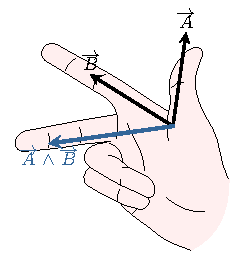
\includegraphics[width=0.25\linewidth]{regle_de_la_main_droite}
		\caption{Schéma de la règle de main droite.}
		\label{fig:regledelamaindroite}
	\end{figure}
	 
	\end{itemize}

	\FloatBarrier

	\subsection*{Q1 Produit Vectoriel}
	Dans la Figure \ref{fig:vector_product_in_space}, le vecteur $\vec{B}$ est aligné vers $\vec{u}_y$ et $\vec{A}$ se trouve dans le plan formé par $\vec{u}_x$ et $\vec{u}_y$. 
	\begin{enumerate}[a)]
	\item Dessiner le vecteur $\vec{C} = \vec{A}  \wedge \vec{B}$ dans la Figure \ref{fig:vector_product_in_space} (la taille de la flèche n'est pas important).
	\item Calculer $\|\vec{C}\|$ en sachant que $\|\vec{B}\| = 1$ et en fonction des constants de la figure?
	\item Calculer $\vec{A}$ en fonction de $h$ et $\theta$.
	\item Calculer $\vec{C}$ avec l'expression du produit vectoriel et vérifier que $\|\vec{C}\|$ correspond au résultat trouvé dans b).
	\item En prenant $\vec{D} = D_x \vec{u}_x$, calculer la valeur de $D_x$ tel que $\vec{B} \wedge \vec{D} = -2 \vec{C}$.
	\item Dans le plan x-z de la Figure \ref{fig:plan_xz}, dessiner les vecteurs $\vec{u}_y$, $\vec{B}$, $\vec{C}$, $\vec{D}$ et $\vec{B} \wedge \vec{D}$. Utilisez respectivement les notations $\otimes$ ou $\odot$ pour représenter un vecteur qui rentre ou qui sort du plan de feuille.
	\end{enumerate}
	
	\begin{figure}
		\centering
	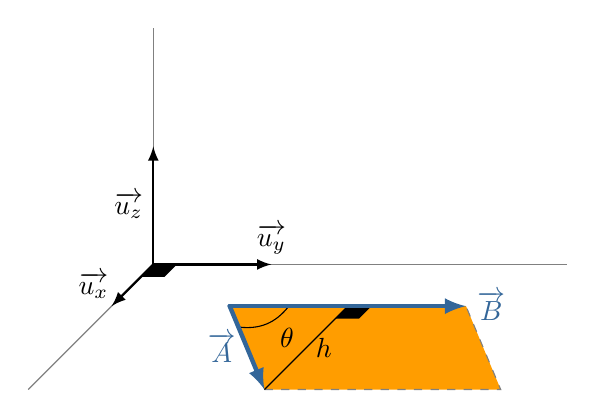
\begin{tikzpicture} [scale=1.5,x={(-0.353cm,-0.353cm)}, y={(1cm,0cm)}, z={(0cm,1cm)}]
		\coordinate (O) at (0, 0, 0);
		\coordinate (A) at (1,1,0);
		\coordinate (B) at (3,2,0);
		\coordinate (C) at (3,4,0);
		\coordinate (D) at (1,3,0);
		\coordinate (E) at (1,2,0);
		%axes et vecteurs unitaires  et définition de x,y,z
		\draw[gray,thin] (O) -- +(3, 0,   0) ;
		\draw[gray,thin] (O) -- +(0,  3.5, 0) ;
		\draw[gray,thin] (O) -- +(0,  0, 2) ;
		\draw[vecteur] (O)-- ++(1,0,0)node[midway,left=5pt]{$\overrightarrow{{u}_{x}}$};
		\draw[vecteur] (O)-- ++(0,1,0)node[above]{$\overrightarrow{{u}_{y}}$};
		\draw[vecteur] (O)-- ++(0,0,1)node[midway,left]{$\overrightarrow{{u}_{z}}$};
		\fill[black](O)--++(.3,0,0)--(.3,.2,0)--(0,.2,0)--cycle;
		% parallelogramme
		\fill[monOrange](A)--(B)--(C)--(D);
		\draw[gray,dashed](B)--(C)--(D);
		\draw[thin](B)--(E)node[midway,right]{$h$};
		\draw[thin](1.5,1.25,0) to[bend right] (1,1.5,0);
		\draw (1.75,1.75,0)node{$\theta$};
		\fill[black](E)--++(.3,0,0)--++(0,.2,0)--++(-.3,0,0)--cycle;
		% vecteurs
		\draw[force] (A)--(B)node[midway,left]{$\overrightarrow{A}$};
		\draw[force] (A)--(D)node[right]{$\overrightarrow{B}$};
		%\draw[force] (A)--++(0,0,2)node[right]{$\overrightarrow{C}$};
	\end{tikzpicture} 
		\caption{}
		\label{fig:vector_product_in_space}
	\end{figure}
	
	\begin{figure}
	\centering	
	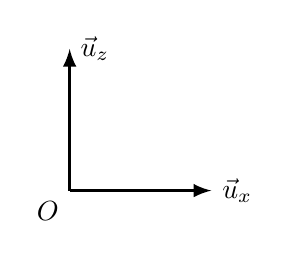
\begin{tikzpicture}
		\coordinate (O) at (0,0);
		\coordinate (X) at (1.8,0);
		\coordinate (Y) at (0,1.8);
		\coordinate (R) at (-0.6, 1.5);
		\coordinate (T) at (1.5, 0.6);	
		\draw[very thick,->] node[below left]{$O$} (O)--(X) node[right]{$\vec{u}_{x}$};
		\draw[very thick,->](O)--(Y) node[right]{$\vec{u}_{z}$};
	\end{tikzpicture}
		\caption{}
		\label{fig:plan_xz}
	\end{figure}
	
	\FloatBarrier
	
	\subsection*{Q2 : Un esquimau sur un igloo}
	Un enfant esquimau joue sur le toit de son igloo. L’enfant se laisse glisser sans frottement depuis le sommet S de l’igloo qui a la forme d’une demi-sphère de rayon $R$ et de centre $O$. La position de l'enfant, assimilé à un point matériel $M$ de masse $m$ est repérée par l’angle $\theta$ par rapport à $\vec{u}_x$. La norme de l'accéleration de la pesanteur est dénoté $g$ (le vecteur $\Vec{g}$ pointe vers le bas). On va étudier ce mouvement en repère polaire. A l’instant initial $t = 0$, l’enfant est situé au sommet de l’igloo et a une vitesse nulle. L’enfant se laisse alors glisser sans frottement sur le toit
	de l’igloo. Ce mouvement s’effectue entièrement $Oxy$. Les objectifs de cet exercice est d'étudier le mouvement en repère de Frénet (vous avez déjà étudié ce mouvement en repère polaire en mécanique du point 1). 
	%trouver la position, c’est à dire l’angle $\theta$, pour laquelle1 l’enfant perd le contact avec l’igloo et l’évolution de la vitesse de l’enfant.
	\begin{enumerate}
	\item Complétez la Figure \ref{fig:igloo} ci-dessous en plaçant $\vec{T}$, $\vec{N}$ et $\vec{B}=\vec{T}\wedge \vec{N}$ (Obs: ($\vec{T}$, $\vec{N}$, $\vec{B}$) forme un base orthonormée direct).
	\begin{figure}[h!]
		\centering
		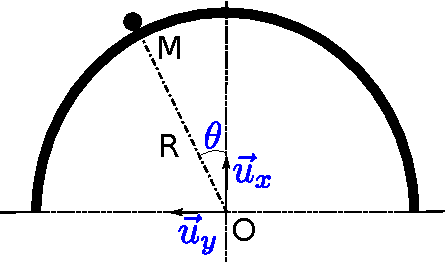
\includegraphics[width=0.4\linewidth]{igloo}
		\caption{Igloo}
		\label{fig:igloo}
	\end{figure}

 	\FloatBarrier
	\item Donner les expressions de toutes les forces en repère de Frénet.
	\item Calculer les moments de chacune de ces forces par rapport au point $O$.
	\item Calculer le moment cinétique de l'enfant par rapport au point $O$.
	\item Appliquer le théorème du moment cinétique à ce mouvement.
	\item Appliquer le principe fondamentale de la dynamique (PFD) en repère de Frénet.
	\item L'équation différentiel trouvé par projection du PFD sur l'axe $\vec{T}$ est-il la même que celle de 5)? Pourquoi? 
	\item Trouver la norme de la vitesse dans l'instant que l'énfant décolle d'igloo (obs: utilisez une des équations du PFD).
	\item L'application du PFD en repère polaire résulte dans les système:
	\begin{align}
		\begin{cases}
			-m g \cos \theta + R_N = -m R \dot{\theta}^2 , \\
			m g \sin \theta = m R \ddot{\theta}
		\end{cases}
	\end{align}
 	Montrer ces équations a partir des résultats de 6).
\end{enumerate}
\end{document}
